\documentclass{standalone}
\usepackage{tikz,pgfplots}
\usepackage{newtxmath}

% definitions for interference images
\colorlet{wall}{blue!30!black}
\colorlet{myblue}{blue!70!black}
\colorlet{myorange}{orange!90!black!80}
\colorlet{myred}{red!70!black}
\colorlet{mydarkred}{red!50!black}
\colorlet{mylightgreen}{green!60!black!70}
\colorlet{mygreen}{green!60!black}
\colorlet{myredgrey}{red!50!black!80}
\colorlet{myshadow}{blue!30!black!90}
\tikzstyle{wave}=[myblue,thick]

\begin{document}

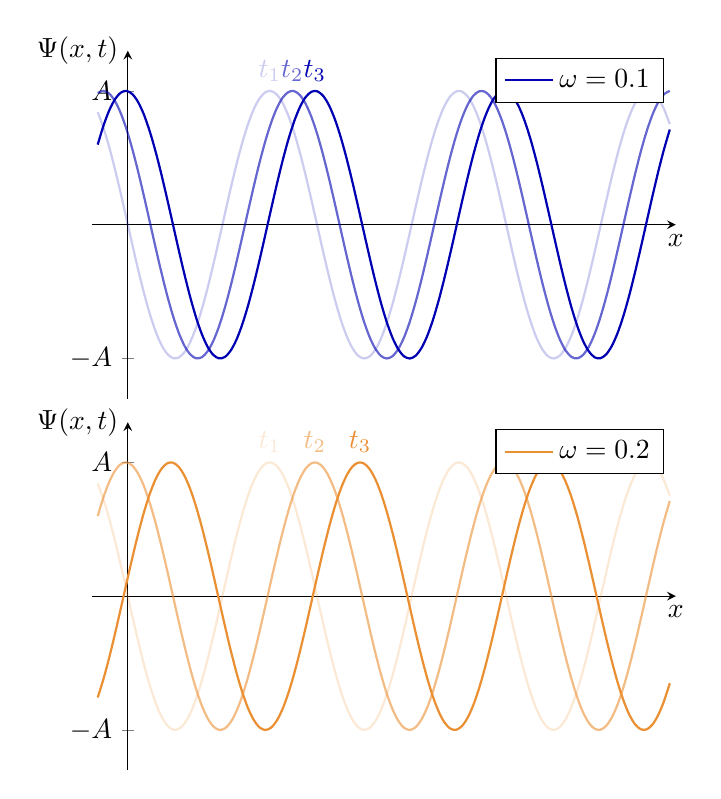
\begin{tikzpicture}
        \begin{axis}[name=plotA,
                    xtick=\empty,
                    ytick={-1,1},
                    yticklabels={$-A$,$A$},
                    axis lines=middle,
                    enlarge x limits={abs=0.2},
                    enlarge y limits={abs=0.3},
                    x label style={anchor=north},
                    y label style={anchor=east},
                    xlabel={$x$},
                    ylabel={$\Psi(x,t)$},
                    width=9cm,
                    height=6cm]
        \addplot[domain=-1:18,samples=100,smooth,myblue,thick] {sin(deg(0.1*15-x))};
        \addplot[domain=-1:18,samples=100,smooth,myblue,thick,opacity=0.2] {sin(deg(0.1*0-x))};
        \addplot[domain=-1:18,samples=100,smooth,myblue,thick,opacity=0.6] {sin(deg(0.1*7.5-x))};
        \addlegendentry{$\omega=0.1$}
        \node[myblue,opacity=0.2] at (axis cs:3*pi/2,1.15) {$t_1$};
        \node[myblue,opacity=0.6] at (axis cs:3*pi/2+0.1*7.5,1.15) {$t_2$};
        \node[myblue] at (axis cs:3*pi/2+0.1*15,1.15) {$t_3$};
        \end{axis}
    
        \begin{axis}[name=plotB,
                    at=(plotA.outer south west),
                    anchor=outer north west,
                    xtick=\empty,
                    ytick={-1,1},
                    yticklabels={$-A$,$A$},
                    axis lines=middle,
                    enlarge x limits={abs=0.2},
                    enlarge y limits={abs=0.3},
                    x label style={anchor=north},
                    y label style={anchor=east},
                    xlabel={$x$},
                    ylabel={$\Psi(x,t)$},
                    width=9cm,
                    height=6cm]
        \addplot[domain=-1:18,samples=100,smooth,myorange,thick] {sin(deg(0.2*15-x))};
        \addplot[domain=-1:18,samples=100,smooth,myorange,thick,opacity=0.2] {sin(deg(0.2*0-x))};
        \addplot[domain=-1:18,samples=100,smooth,myorange,thick,opacity=0.6] {sin(deg(0.2*7.5-x))};
        \addlegendentry{$\omega=0.2$}
        \node[myorange,opacity=0.2] at (axis cs:3*pi/2,1.15) {$t_1$};
        \node[myorange,opacity=0.6] at (axis cs:3*pi/2+0.2*7.5,1.15) {$t_2$};
        \node[myorange] at (axis cs:3*pi/2+0.2*15,1.15) {$t_3$};
        \end{axis}
    \end{tikzpicture}

\end{document}